\documentclass{beamer}

\usepackage{beamerthemesplit}
\usepackage{graphicx}
\usepackage{color, natbib, hyperref}
\usepackage{bibentry}
\nobibliography*

% Algorithm environment
\usepackage{algpseudocode,algorithm,algorithmicx}
\newcommand*\Let[2]{\State #1 $\gets$ #2}


% define colors
\definecolor{jblue}  {RGB}{20,50,100}
\definecolor{ngreen} {RGB}{98,158,31}

%theme

\usetheme{boxes} 
%\usecolortheme{seahorse} 
\setbeamertemplate{items}[default] 
%\setbeamercovered{transparent}
\setbeamertemplate{blocks}[rounded]
\setbeamertemplate{navigation symbols}{} 
% set the basic colors
\setbeamercolor{palette primary}   {fg=black,bg=white}
\setbeamercolor{palette secondary} {fg=black,bg=white}
\setbeamercolor{palette tertiary}  {bg=jblue,fg=white}
\setbeamercolor{palette quaternary}{fg=black,bg=white}
\setbeamercolor{structure}{fg=jblue}
\setbeamercolor{titlelike}         {bg=jblue,fg=white}
\setbeamercolor{frametitle}        {bg=jblue!10,fg=jblue}
\setbeamercolor{cboxb}{fg=black,bg=jblue}
\setbeamercolor{cboxr}{fg=black,bg=red}

% reduce space before/after equations
\expandafter\def\expandafter\normalsize\expandafter{%
    \normalsize
    \setlength\abovedisplayskip{1pt}
    \setlength\belowdisplayskip{1pt}
    \setlength\abovedisplayshortskip{1pt}
    \setlength\belowdisplayshortskip{1pt}
}

% set colors for itemize/enumerate
\setbeamercolor{item}{fg=ngreen}
\setbeamercolor{item projected}{fg=white,bg=ngreen}

% set colors for blocks
\setbeamercolor{block title}{fg=ngreen,bg=white}
\setbeamercolor{block body}{fg=black,bg=jblue!10}

% set colors for alerted blocks (blocks with frame)
\setbeamercolor{block alerted title}{fg=white,bg=jblue}
\setbeamercolor{block alerted body}{fg=black,bg=jblue!10}
\setbeamercolor{block alerted title}{fg=white,bg=dblue!70} % Colors of the highlighted block titles
\setbeamercolor{block alerted body}{fg=black,bg=dblue!10} % Colors of the body of highlighted blocks

% set the fonts
\usefonttheme{professionalfonts}

\setbeamerfont{section in head/foot}{series=\bfseries}
\setbeamerfont{block title}{series=\bfseries}
\setbeamerfont{block alerted title}{series=\bfseries}
\setbeamerfont{frametitle}{series=\bfseries}
\setbeamerfont{frametitle}{size=\Large}
\setbeamerfont{block body}{series=\mdseries}
\setbeamerfont{caption}{series=\mdseries}
\setbeamerfont{headline}{series=\mdseries}


% set some beamer theme options
\setbeamertemplate{title page}[default][colsep=-4bp,rounded=true]
\setbeamertemplate{sections/subsections in toc}[square]
\setbeamertemplate{items}[circle]
\setbeamertemplate{blocks}[width=0.0]
\beamertemplatenavigationsymbolsempty

% Making a DAG
\usepackage{tkz-graph}  
\usetikzlibrary{calc}
\usetikzlibrary{shapes.geometric}
\usetikzlibrary{positioning}
\tikzstyle{VertexStyle} = [shape            = rectangle,
                               minimum width    = 6ex,%
                               draw]
 \tikzstyle{EdgeStyle}   = [->,>=stealth']      

% Define block styles
\tikzstyle{f} = [rectangle, draw, fill=blue!20, 
    text width=3em, text badly centered, node distance=1.75cm]
\tikzstyle{message} = [rectangle, draw, fill=green!20, 
    text width=3em, text centered]
\tikzstyle{io} = [draw, circle,fill=red!20, node distance=2cm,
    minimum height=2em]
\tikzstyle{line} = [draw, -latex']

% Math macros
\newcommand{\cD}{{\mathcal D}}
\newcommand{\cF}{{\mathcal F}}
\newcommand{\todo}[1]{{\color{red}{TO DO: \sc #1}}}

\newcommand{\reals}{\mathbb{R}}
\newcommand{\integers}{\mathbb{Z}}
\newcommand{\naturals}{\mathbb{N}}
\newcommand{\rationals}{\mathbb{Q}}

\newcommand{\ind}[1]{1_{#1}} % Indicator function
\newcommand{\pr}{\mathbb{P}} % Generic probability
\newcommand{\ex}{\mathbb{E}} % Generic expectation
\newcommand{\var}{\textrm{Var}}
\newcommand{\cov}{\textrm{Cov}}

\newcommand{\normal}{N} % for normal distribution (can probably skip this)
\newcommand{\eps}{\varepsilon}
\newcommand\independent{\protect\mathpalette{\protect\independenT}{\perp}}
\def\independenT#1#2{\mathrel{\rlap{$#1#2$}\mkern2mu{#1#2}}}

\newcommand{\convd}{\stackrel{d}{\longrightarrow}} % convergence in distribution/law/measure
\newcommand{\convp}{\stackrel{P}{\longrightarrow}} % convergence in probability
\newcommand{\convas}{\stackrel{\textrm{a.s.}}{\longrightarrow}} % convergence almost surely

\newcommand{\eqd}{\stackrel{d}{=}} % equal in distribution/law/measure
\newcommand{\argmax}{\arg\!\max}
\newcommand{\argmin}{\arg\!\min}

\newcommand{\bit}{\begin{itemize}}
\newcommand{\eit}{\end{itemize}}


\mode<presentation>

\title[Simple Random Sampling: Not So Simple]{Simple Random Sampling: Not So Simple}
\author{Kellie Ottoboni \\ with Philip B.~Stark and Ron Rivest}
\institute[]{Department of Statistics, UC Berkeley\\Berkeley Institute for Data Science}
\date{Qualifying Exam \\ January 23, 2017}

\begin{document}

\frame{
\titlepage
\vfill
\begin{columns}[T]
\begin{column}{.5\textwidth}
\begin{center}
\vspace{25pt}

\includegraphics[width=\textwidth]{fig/logo/dept1.pdf}
\end{center}
\end{column}
\begin{column}{.3\textwidth}
\begin{center}
\end{center}
\end{column}
\begin{column}{.3\textwidth}
\begin{center}

\includegraphics[width=0.9\textwidth]{fig/logo/BIDS.png}
\end{center}
\end{column}
\end{columns}
}


\section[Introduction]{Introduction}


\frame{
\begin{figure}[htbp]
\begin{center}
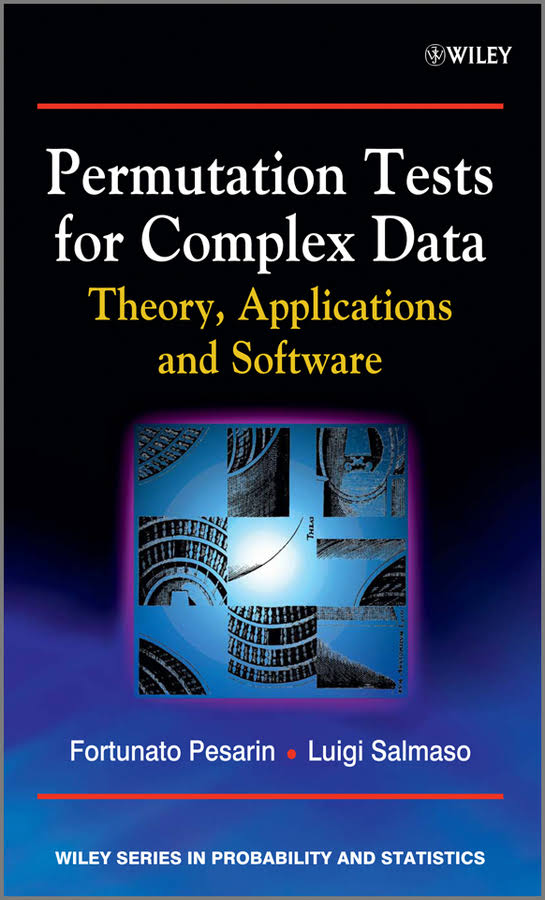
\includegraphics[height = .8\textheight]{fig/book}
\end{center}
\end{figure}
}

\frame{
\frametitle{Simple Random Sampling}
\textbf{Simple random sampling:} drawing $k$ objects from a group of $n$ in such a way that all $n\choose k$ possible subsets are equally likely \\
\vspace{15pt}

If there is a problem generating SRSs, it will be even worse for other methods: permutation, bootstrap samples, MCMC, Monte Carlo integration...

\begin{table}[htdp]
{Number of possibilities for $n = 100$, $k = 50$}
\begin{center}
\begin{tabular}{l|c|c}
\hline
SRSs & $n \choose k$ & ${100 \choose 50} \approx 10^{29}$ \\
Bootstrap Samples& $n^k$ & $100^{50} = 10^{100}$ \\
Permutations & $n!$ & $100! \approx 10^{158}$ \\
\hline 
\end{tabular}
\end{center}
\end{table}%

}

\frame{
\frametitle{Simple Random Sampling}
In practice, it is difficult to draw truly random samples.
\vspace{20pt}

Instead, people tend to draw samples using
\bit
\item A \textbf{pseudorandom number generator} (PRNG) that produces sequences of bits
\item An algorithm that maps a set of pseudorandom numbers into a subset of the population
\eit
\vspace{20pt}

Most people take for granted that this procedure is a sufficient approximation to simple random sampling.
}


\frame{
\frametitle{PRNGs}

A PRNG is a deterministic function with several components:
\bit
\item A user-supplied seed value used to set the internal state
\item A function that maps the internal state to random bits
\item A function that updates the internal state 
\eit

\begin{center}
\resizebox{10cm}{!}{    
\begin{tikzpicture}[node distance = 3cm, auto, scale = 0.5]
    % Place nodes
    \node[io] (seed) {Seed};
    \node [f, right of=seed, node distance = 3cm] (state) {Internal state};
    \node [message, right of=state, node distance = 3cm] (output) {Random bits};
    % Draw edges
    \path [line] (seed) -- (state);
    \path [line] (state) -- (output);
    \path (state) edge [->, in = 130, out = 50, distance = 20mm] node[above] {Update} (state);
    % Draw box 
    \draw ($(state.north west)+(-2.5,2.5)$)  rectangle ($(state.south east)+(2.5,-1)$);
\end{tikzpicture}
}
\end{center}

}


\frame{
\frametitle{Pigeons and Pigeonholes}

\begin{theorem}[Pigeonhole Principle]
If there are $n$ pigeonholes and $m>n$ pigeons, then there exists at least one pigeonhole containing more than one pigeon.
\end{theorem}
\begin{figure}[htbp]
\begin{center}
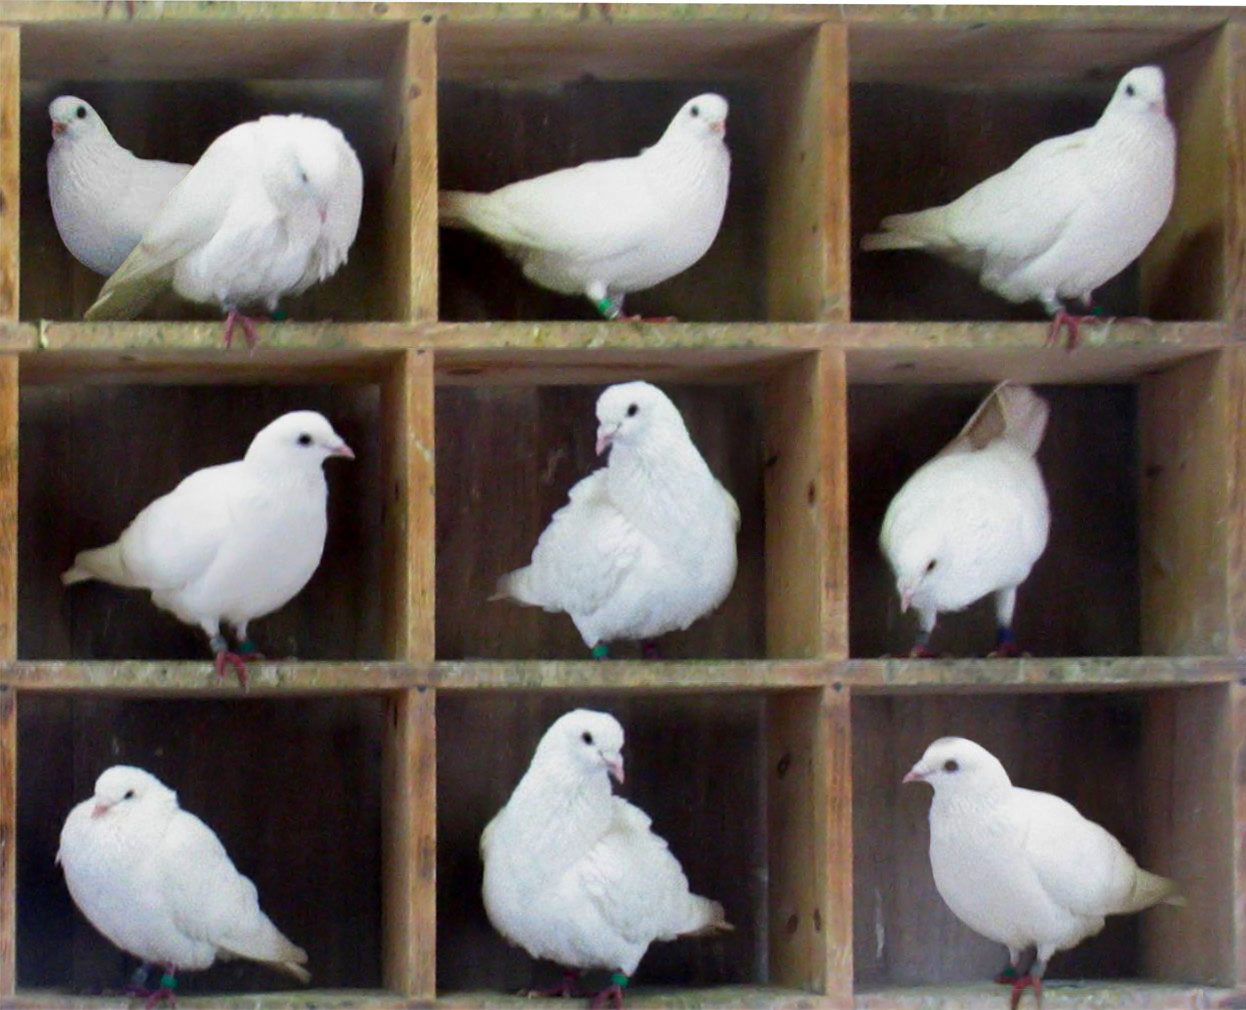
\includegraphics[width = .3\textwidth]{fig/TooManyPigeons.jpg}
\end{center}
\tiny \href{https://commons.wikimedia.org/w/index.php?curid=4658682}{(Wikipedia)}
\end{figure}

\pause
\begin{corollary}[Too few pigeons]
If ${n \choose k}$ is greater than the size of a PRNG's state space, then the PRNG cannot possibly generate all samples of size $k$ from a population of $n$.
\end{corollary}
}


\frame{
\frametitle{Pigeons and Pigeonholes}

Period of 32-bit linear congruential generators: \\
\setlength{\parindent}{10ex} at most $2^{32} \approx 4 \times 10^9$ \\
% (some poorly designed ones have an even shorter period) \\
\noindent Samples of size $10$ from $50$: \\
${50 \choose 10} \approx 10^{10}$ \\
\noindent \textbf{More than half of samples cannot be generated}
\vspace{20pt}
\pause

\noindent Period of Mersenne Twister (standard PRNG in Statistics): \\
$2^{32 \times 624} \approx 2 \times 10^{6010}$ \\
\noindent Permutations of $2084$ objects: \\
$2084! \approx 3 \times 10^{6013}$\\
\noindent\textbf{Less than $0.01\%$ of permutations can be generated}
}


\begin{frame}[label = pigeonhole]
\frametitle{Pigeons and Pigeonholes}
But does it \textit{really} matter in practice?

\bit
\itemsep10pt
\item Social applications may require the PRNG to produce all possible samples -- e.g. jury duty summons, gaming machines, lottery tickets (\cite{marsaglia_seeds_2003})
\item \todo{think about if I want to include this} Impossibility bounds show that some statistics estimated from Monte Carlo distributions will have nontrivial bias (though we don't know which statistics) \hyperlink{impossibility_bounds}{\beamerbutton{here}}
\eit
\end{frame}



\frame{
\frametitle{Arguments}
\bit
\item Some sampling algorithms are better than others -- look under the hood of your software
\item Inputs to your PRNGs matter for producing ``good'' PRNs
\item PRNGs for Statistical applications should be judged on how well they produce random samples when passed into a reasonable sampling algorithm
\eit
}


\section[Sampling algorithms]{Sampling Algorithms}
  \begin{frame}
  \frametitle{Contents}
  \tableofcontents[currentsection]
  \end{frame}
  
  
  
\frame{
\frametitle{Sampling Algorithms}

Given a sequence of (pseudo)random numbers, how do we use them to draw a SRS? \\
\vspace{15pt}
Two general strategies:
\bit
\item ``Shuffle the deck'' and take the top $k$ as the sample
\item Number the population, select $k$ random integers, and take the corresponding items
\eit
}

\frame{
\frametitle{PIKK}
\begin{algorithm}[H]                      % enter the algorithm environment
\caption{PIKK: Permute indices and keep $k$}          % give the algorithm a caption
\label{PIKK}                           % and a label for \ref{} commands later in the document
\begin{algorithmic}[1]             % enter the algorithmic environment
     \State{Assign IID uniform values on $[0,1]$ to the $n$ elements of the population}
     \State{Sort the population according to these values (break ties randomly)}
     \State{Take the top $k$ to be the sample}
\end{algorithmic}
\end{algorithm}

\bit
\item Relies on assumption that all permutations are equally likely
\item Inefficient: requires $n$ PRNs and $O(n\log n)$ sorting operation
\item Possibly the basis for the \texttt{sample} function in Stata
\eit

\todo{who else recommends PIKK? do a lit search}

}




\frame{
\frametitle{Shuffling algorithms}
\bit
\item Knuth shuffle: requires $n-1$ random integers, but no sorting. This is what \texttt{np.random.choice} does.
\begin{algorithm}[H]                      % enter the algorithm environment
\caption{Fisher-Yates-Knuth-Durstenfeld shuffle}          % give the algorithm a caption
\label{FYKD}                           % and a label for \ref{} commands later in the document
\begin{algorithmic}[1]               % enter the algorithmic environment
\For{$i = 2, \dots, n$}
    \Let{$J$}{random integer uniformly distributed on $1, \dots, i$}
    \Let{$(a[J], a[i])$}{$(a[i], a[J])$}
\EndFor
\State{Take the first $k$ to be the sample}
\end{algorithmic}
\end{algorithm}
\todo{put proof that shuffle works in appendix}
\item Reservoir algorithms: Algorithm R (Waterman, Knuth 1997), Algorithm Z (Vitter 1985) are related to shuffling and don't require knowing the population size a priori
\eit
}


\frame{
\frametitle{Random indices}
\begin{algorithm}[H]                      % enter the algorithm environment
\caption{Uniform random indices}          % give the algorithm a caption
\label{algo:uri}                           % and a label for \ref{} commands later in the document
\begin{algorithmic}[1]             % enter the algorithmic environment
\Let{$\tilde{n}$}{$n$}
\Let{Population indices}{$\{1, \dots, n\}$}
\For{$i = 1, \dots, k$}
%     \Let{$w$}{a uniform PRN on $[0, 1)$}
%     \Let{$j$}{Element in the $\lfloor\tilde{n}w\rfloor + 1$ space in Population indices}
     \Let{$w$}{A random integer on $\{1, \dots, \tilde{n}\}$}
     \Let{$j$}{The $w$th element in Population indices}
     \Let{Sample indices}{Sample indices $\cup \{j\}$}
     \Let{Population indices}{Put last remaining index in place $w$}
     \Let{$\tilde{n}$}{$\tilde{n}-1$}
\EndFor
\State{Take the items with selected Sample indices}
\end{algorithmic}
\end{algorithm}

\bit
\item Method used by R \texttt{sample}, Python \texttt{random.sample}
\item More efficient: uses only $k$ PRNs and no sorting
\eit
}


\begin{frame}[label = nonuniform-lemma]
\frametitle{Generating (non)uniform integers}
\bit
\item These algorithms depend on uniformly distributed integers
\item A common way to get integers in the range $\{1, \dots, m\}$ is $X = \lfloor m U\rfloor + 1$, $U \sim U[0,1)$.
%\bit
%\item $U$ is uniform on $\{0, 2^{-w}, 2\times 2^{-w}, \dots, (2^w - 1)\times2^{-w}\}$
%\item $mU$ is uniform on $\{0, m2^{-w}, 2m\times 2^{-w}, \dots, (2^w - 1)m\times2^{-w}\}$
%\eit
\item Unless $m$ is a multiple of $2^w$, $\lfloor mU \rfloor$ will not truly be uniform! (\cite{knuth_art_1997})
\eit

\begin{lemma}
For $m < 2^w$, the ratio of the largest to smallest selection probability is, to first order,  $1+ m 2^{-w}$.
\end{lemma}

\hyperlink{nonuniform-proof}{\beamerbutton{Proof}}

\end{frame}



\frame{
\frametitle{Generating (non)uniform integers}

\bit
\item A better way to generate integers on $\{1, \dots, m\}$:
\vspace{10pt}
 Let \begin{displaymath}
   w = \left\{
     \begin{array}{lr}
       \log_2(m) & \text{if $m$ is a power of 2}\\
       \lfloor \log_2(m) \rfloor + 1 & \text{otherwise}
     \end{array}
   \right.
\end{displaymath} 

\vspace{10pt}

Generate a $w$-bit integer $J$. If $J > m$, discard and repeat.
\vspace{10pt}

\item Possibly slow: will discard nearly half of draws when $m$ is close to $2^{w-1}$
\item Resulting integers will truly be uniform
\eit
}



\frame{
\frametitle{Sampling Algorithms}
\begin{table}[htdp]
\begin{center}
\begin{tabular}{l|c|c}
Package & Sampling algorithm & Random integer algorithm \\
\hline
R & random indices & variant of floor method \\
Python \texttt{random} & random indices & discard method \\
Numpy \texttt{random} & shuffle and keep $k$ & discard method \\
Stata & ? & ? \\
\hline 
\end{tabular}
\end{center}
\end{table}%


\bit
\item Stata blogs recommend people use PIKK when coding up sampling themselves. But Stata's sort function is randomized by default. Not reproducible! (\cite{schumm_stata_2006})
\item \todo{R bug report}
\eit
}

\frame{
\frametitle{Sampling Algorithms}
\todo{May want to remove this slide or move it later}

\bit
\item Generate samples using a single PRNG and single seed, various sampling algorithms and number of samples \todo{what's the seed}
\item Red require $n$ PRNs; Blue require only $k$ PRNs
\item No straightforward pattern in how uniform the samples are
\eit

%\begin{figure}[htbp]
%\begin{center}
%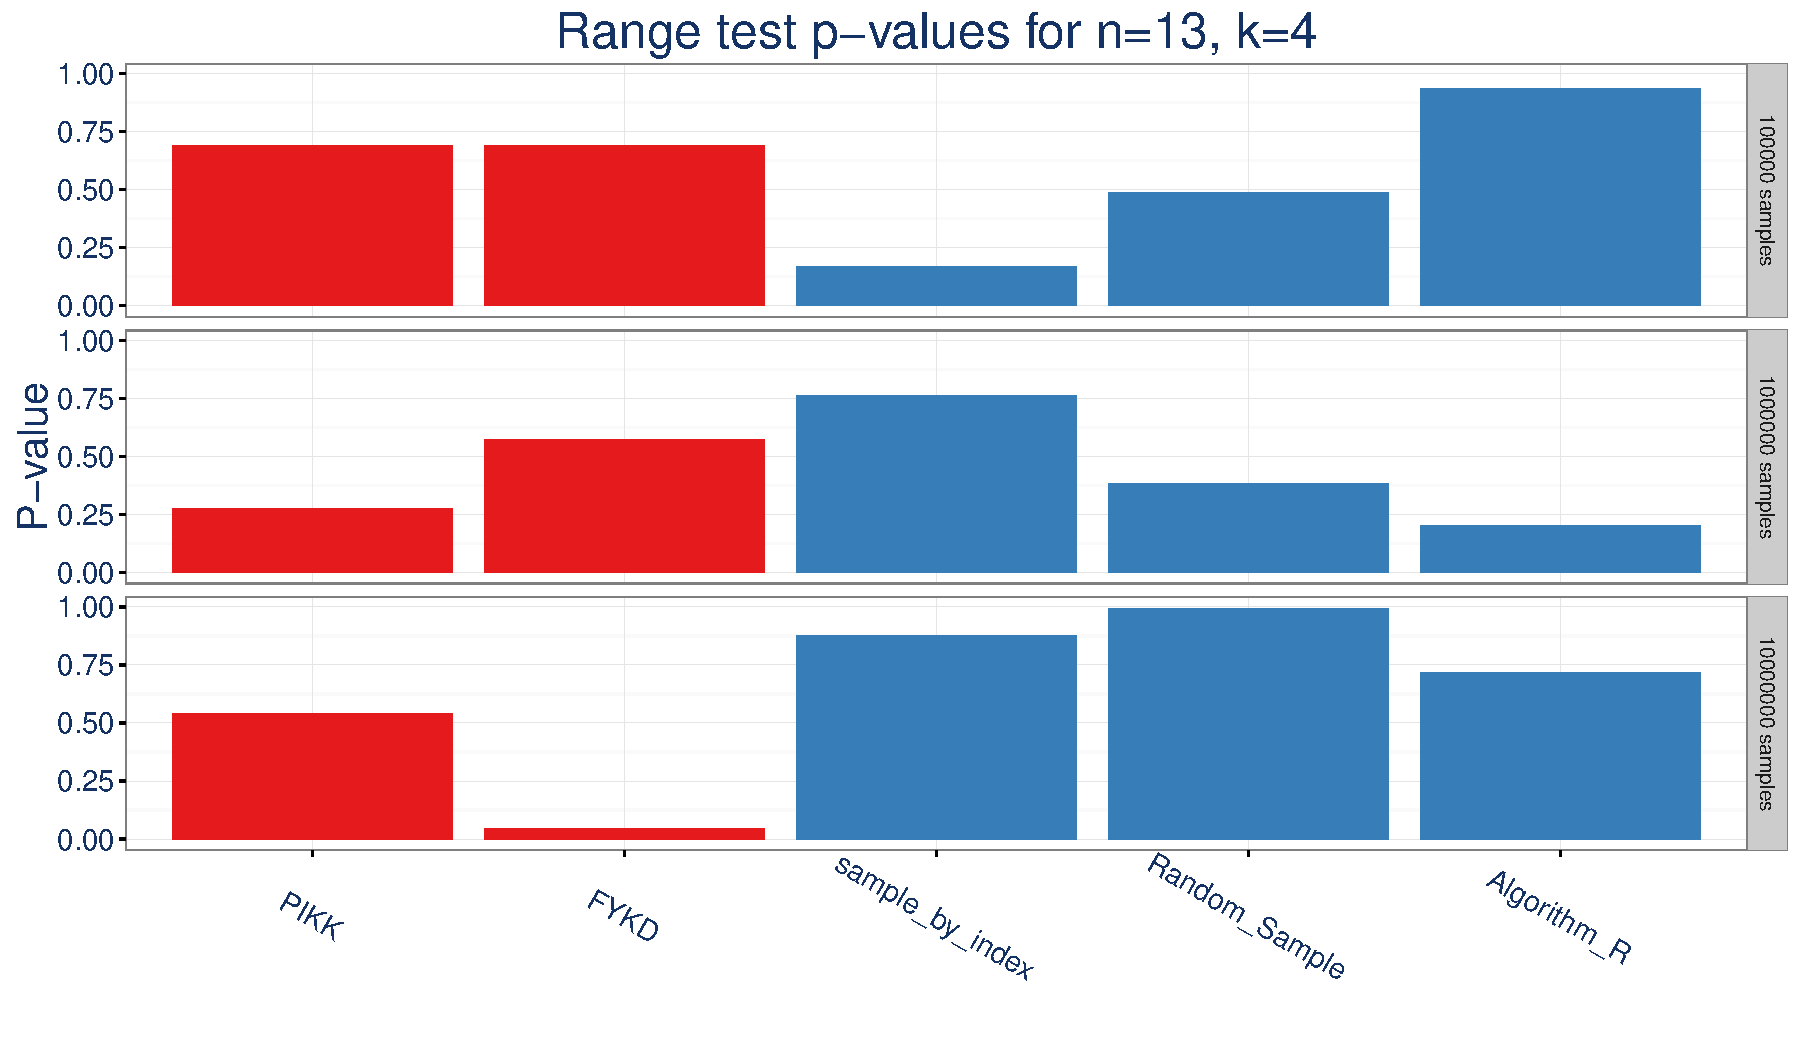
\includegraphics[width = .8\textwidth]{fig/sa-comparison}
%\end{center}
%\end{figure}
\begin{figure}[htbp]
\begin{center}
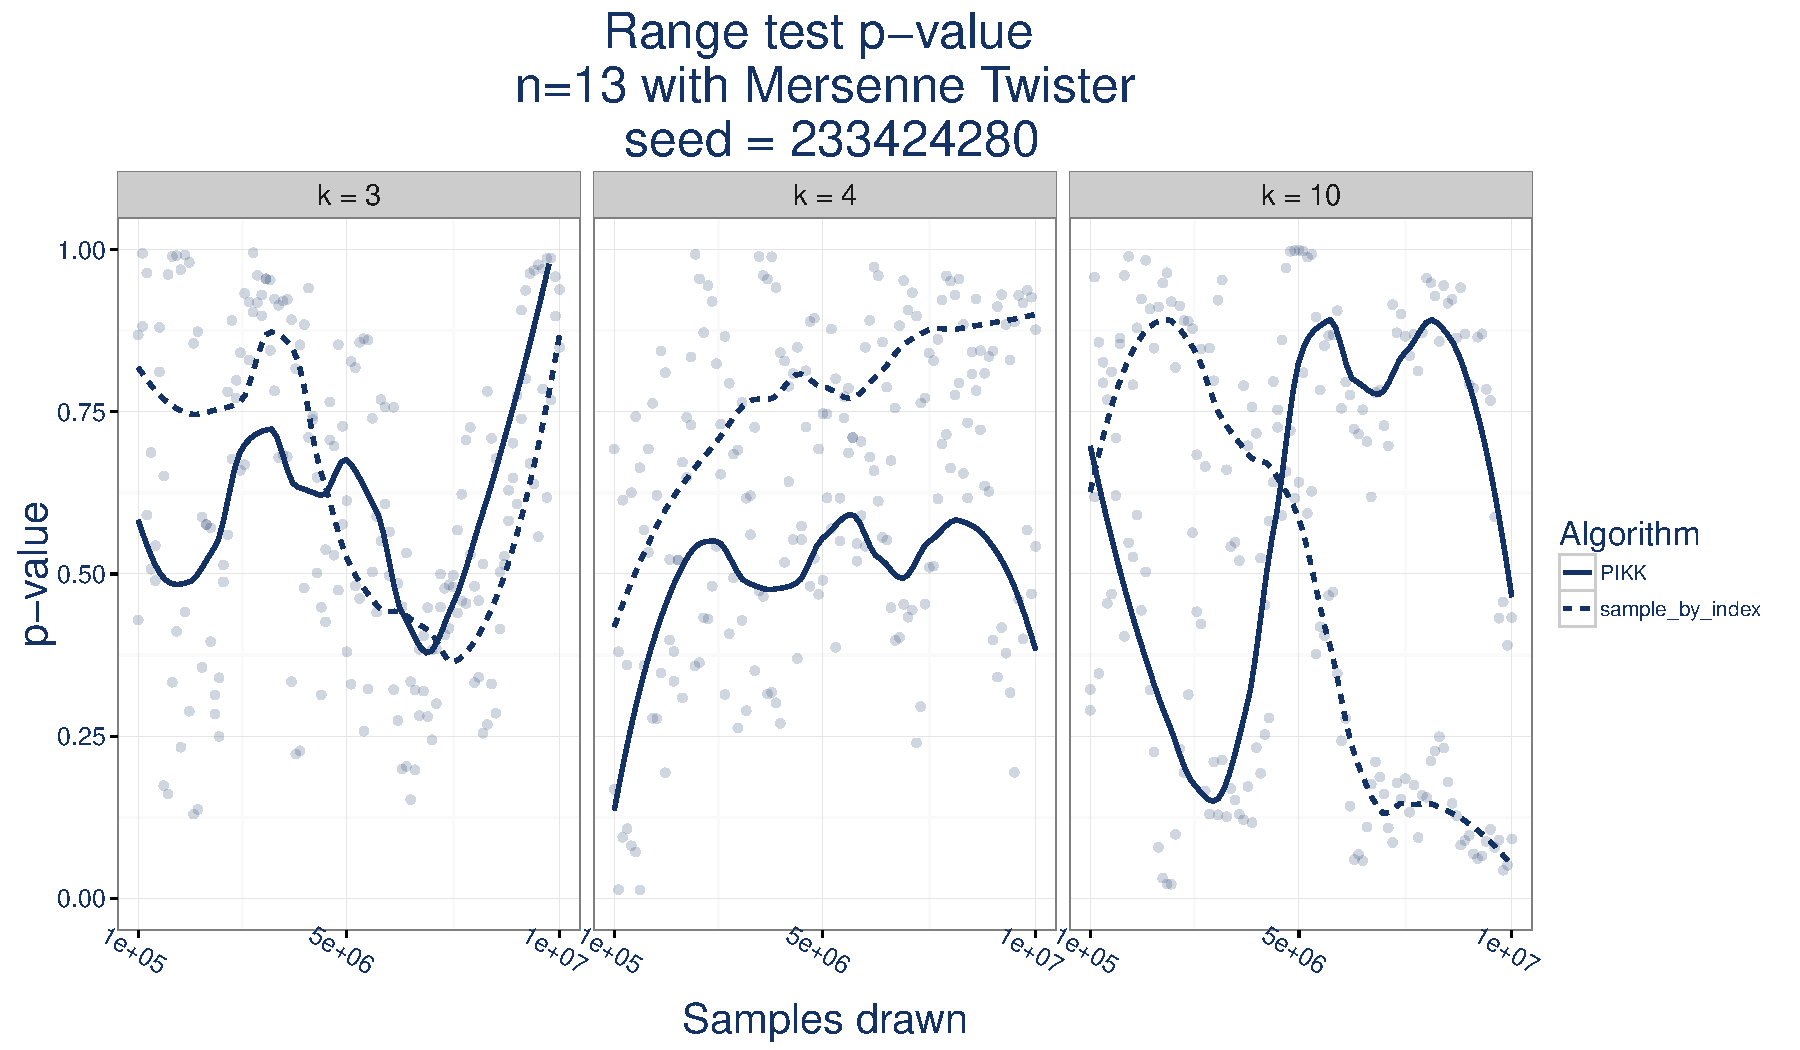
\includegraphics[width = .8\textwidth]{fig/prng-sa-lineplot}
\end{center}
\end{figure}

}

\section[Pseudorandomness]{Pseudorandomness}

  \begin{frame}
  \frametitle{Contents}
  \tableofcontents[currentsection]
  \end{frame}

\frame{
\frametitle{Pseudorandomness}
\begin{figure}[htbp]
\begin{center}
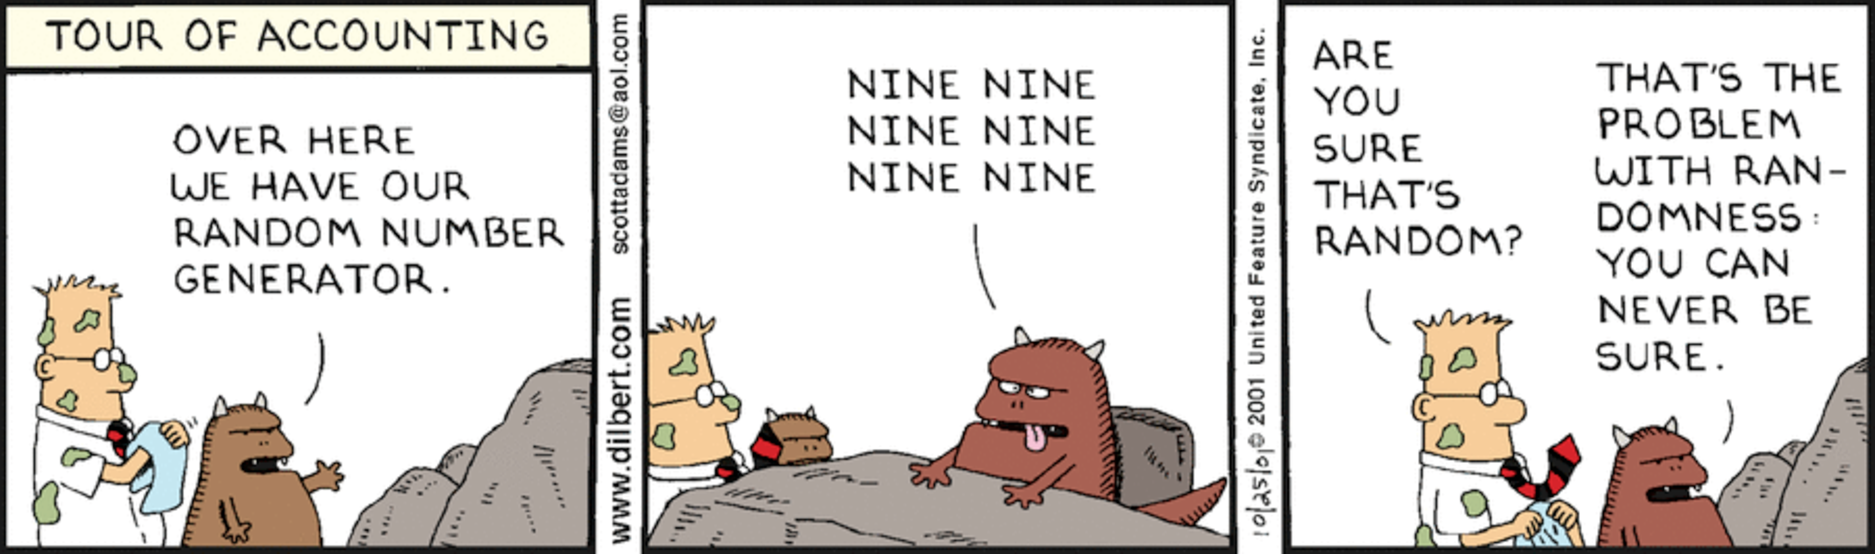
\includegraphics[width = .8\textwidth]{fig/dilbert}
\end{center}
\tiny \href{http://dilbert.com/strip/2001-10-25}{Dilbert}
\end{figure}


\textbf{Pseudorandom}: deterministic, but having the same relevant statistical properties as if random


\bit
\item Uniformity: values and sequences of values should be equiprobable
\item Independence: lack of serial correlation, unpredictable
\eit
\pause
PRNGs can't do this perfectly.
\bit
\item They are deterministic. Knowing input tells you the output.
\item Most are \textbf{periodic}: they eventually produce the same sequence of values.
\item They have some predictable mathematical structure.
\eit
}



\frame{
\frametitle{What makes a PRNG}

\bit
\item Mimics a random sequence (statistically indistinguishable)
\item Unpredictable. This is different from random - if it's deterministic, then it's predictable to some degree
\item Fast and memory efficient
\item Desirable, but not essential:
\bit 
\item Jump-ahead feature to efficiently skip through random numbers, generate multiple streams for parallel applications
\item \todo{}
\eit
\eit
}



\frame{
\frametitle{Testing PRNGs}
\bit
\itemsep 10pt
\item ``Independent'' and ``uniform'' are broad criteria -- many ways to define and check for these properties
\bit
\itemsep 10pt
\item Uniformity at varying levels of granularity
\item Correlations within and between subsequences
\eit
\item Test batteries: 
\bit
\itemsep 10pt
\item Diehard battery (\cite{marsaglia_diehard_1995})
\item NIST Statistical Test Suite (\cite{soto_statistical_1999,rukhin_statistical_2010})
\item TestU01 suite (\cite{lecuyer_testu01_2007})
\eit
\eit
}


\frame{
\frametitle{Testing for uniformity}
\begin{enumerate}
\item Kolmogorov-Smirnov test: values should appear IID $U[0,1]$
\pause
\item Chi-squared test: break values or sequences of values into categories with known frequencies under the null
\pause
\item \textbf{New proposal:} Range test \\

Break values into equally probable categories and compute the range of observed frequencies

$$ R = \max_{i} O_i - \min_i O_i$$

$R$ has a complicated distribution based on multinomial distribution... use asymptotic approximation from \citet{young_two_1962}: 

$$\pr(R \leq r) \approx P(W_N \leq (r-(2B)^{-1})(N/B)^{1/2})$$
where $W_N$ denotes the sample range of $N$ independent standard normal random variables.
\end{enumerate}
}


\frame{
\frametitle{Testing for independence}

\begin{enumerate}
\item Gap test: count length of sequence between values in a given range
\item Permutation test: look at ordering of values in subsequences of length $t$
\item Serial correlation test: correlation between consecutive pairs of values
\item Many more possibilities!
\end{enumerate}

}



\frame{
\frametitle{Geometric tests}
\bit
\item Some PRNGs generate points with geometric structure (more on this later)
\item The \textbf{spectral test} in dimension $d$ considers a set of parallel hyperplanes that covers all points $(x_n, \dots, x_{n+d - 1})$.
$$\nu_d = 1/\max{\text{distance between parallel hyperplanes}}$$
\eit

 Idea: More information needed to describe structure $\iff$ less correlation between consecutive PRNs

\begin{figure}
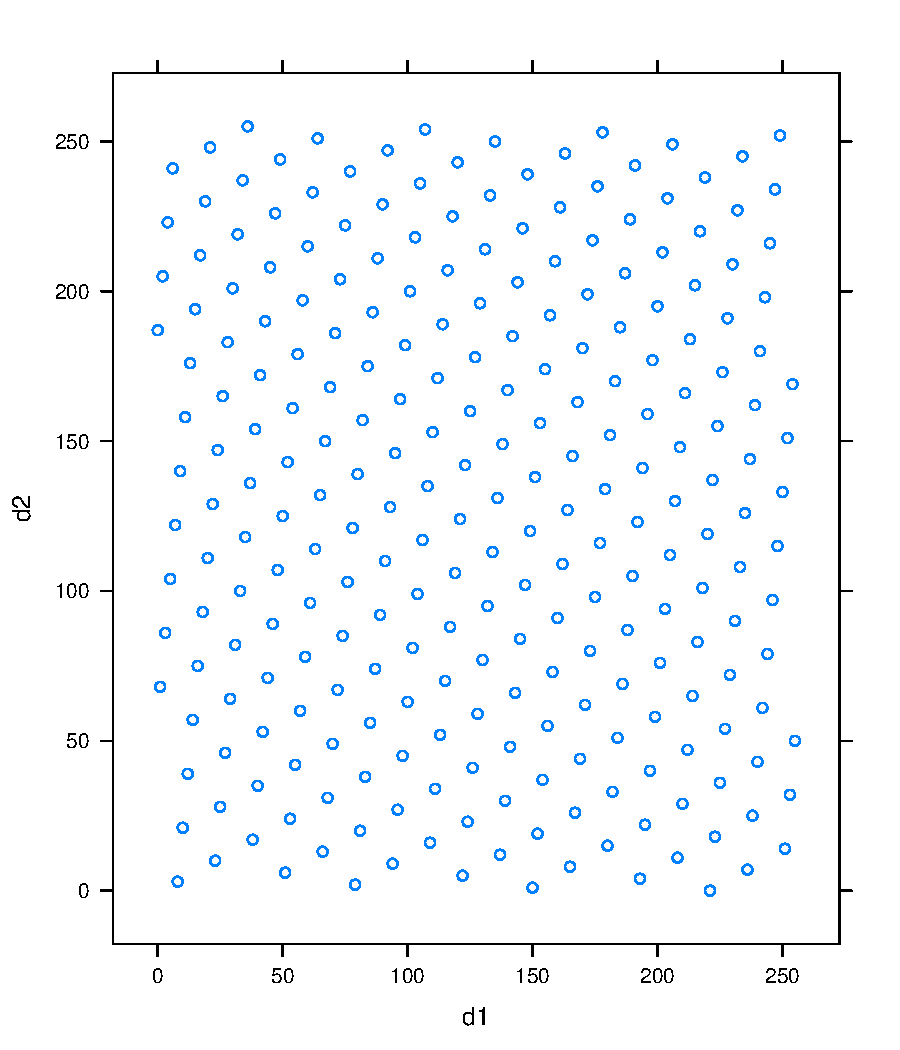
\includegraphics[width = 0.25\textwidth]{fig/lcg_2d}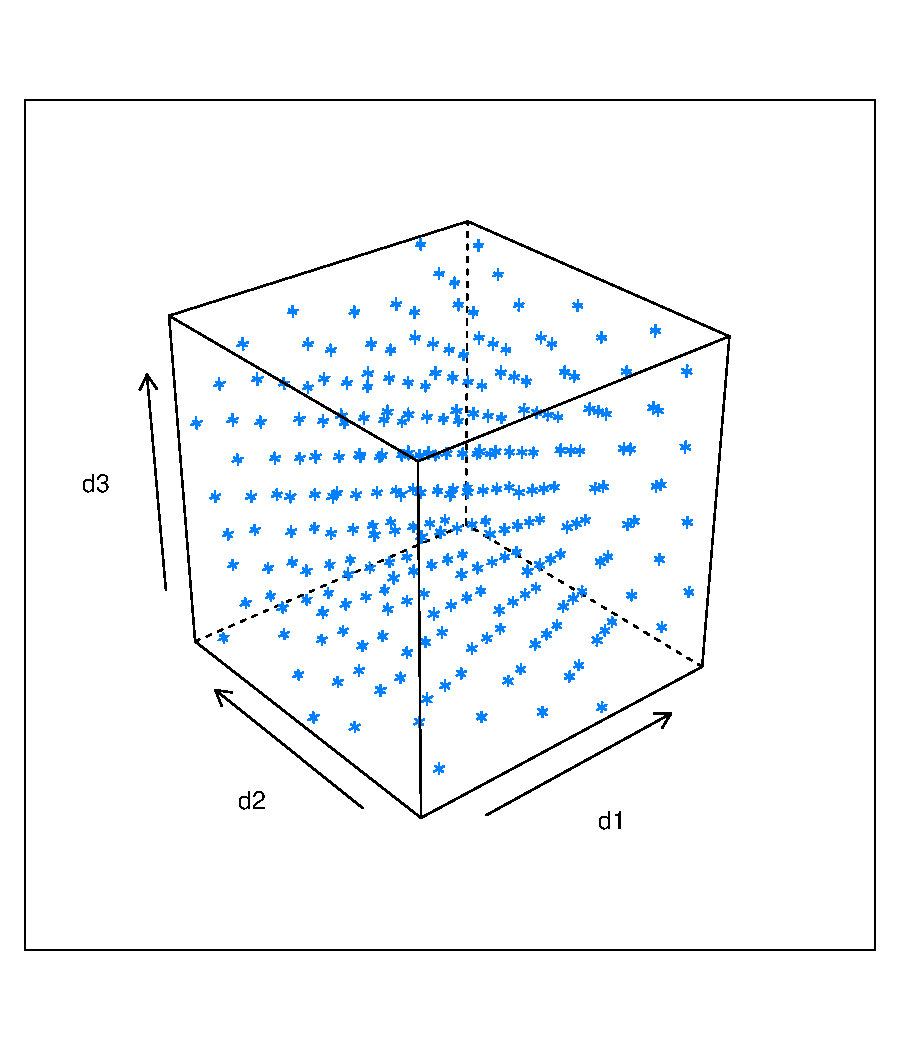
\includegraphics[width = 0.25\textwidth]{fig/lcg_3d} \\
{\tiny $ X_{n+1} = (137X_n+ 187) \mod 256$}
\end{figure}
}



\frame{
\frametitle{Testing PRNGs}

\bit
\item Some sampling algorithms use PRNGs in ways that are not covered by these tests
\item E.g. Algorithm~\ref{algo:uri} for sampling by uniform random indices
\bit
\item To generate a SRS of size $k$ from $n$, obtain PRNs $(U_1, \dots, U_k)$ where 
$U_j$ is uniform on $\{1, \dots, n - j + 1\}$
\item The sequences $(U_1, \dots, U_k)$ should themselves be equiprobable
\eit
\pause
\item Test by generating a large ``sample'' of $B$ SRSs

\begin{align*}
H_0&: \pr(\text{SRS}_i ) = \frac{1}{{n\choose k}} \text{ for all ${n\choose k}$ possible SRSs} \\
H_1&: \pr(\text{SRS}_i ) \neq \frac{1}{{n\choose k}}\text{ for some SRS} 
\end{align*}
\vspace{15pt}


\item Under $H_0$, the number of times each SRS is observed follows a multinomial distribution with $B$ trials and equal selection probabilities $1/{n \choose k}$

\eit
}


\frame{
\frametitle{Testing PRNGs}
Test proposals:

\bit
\item Chi-squared or range test
\item Sequential probability ratio test
\eit
}

\frame{
\frametitle{SPRT}
\todo{}
}

%\frame{
%\frametitle{Bad seeds}
%\bit
%\item \textbf{Seed}: an initial value to set the internal state of a PRNG.
%\item Mersenne Twister has problems with seeds with too many zeros (\cite{saito_simd-oriented_2008})
%\item LCGs may not achieve their full period with certain seeds (\cite{park_random_1988})
%\eit
%
%\todo{Think about removing this and putting in some of the frequency simulation results instead. This is a highly stylized example - I hand picked the seeds, reps, etc}
%
%\pause
%\begin{figure}[htbp]
%\begin{center}
%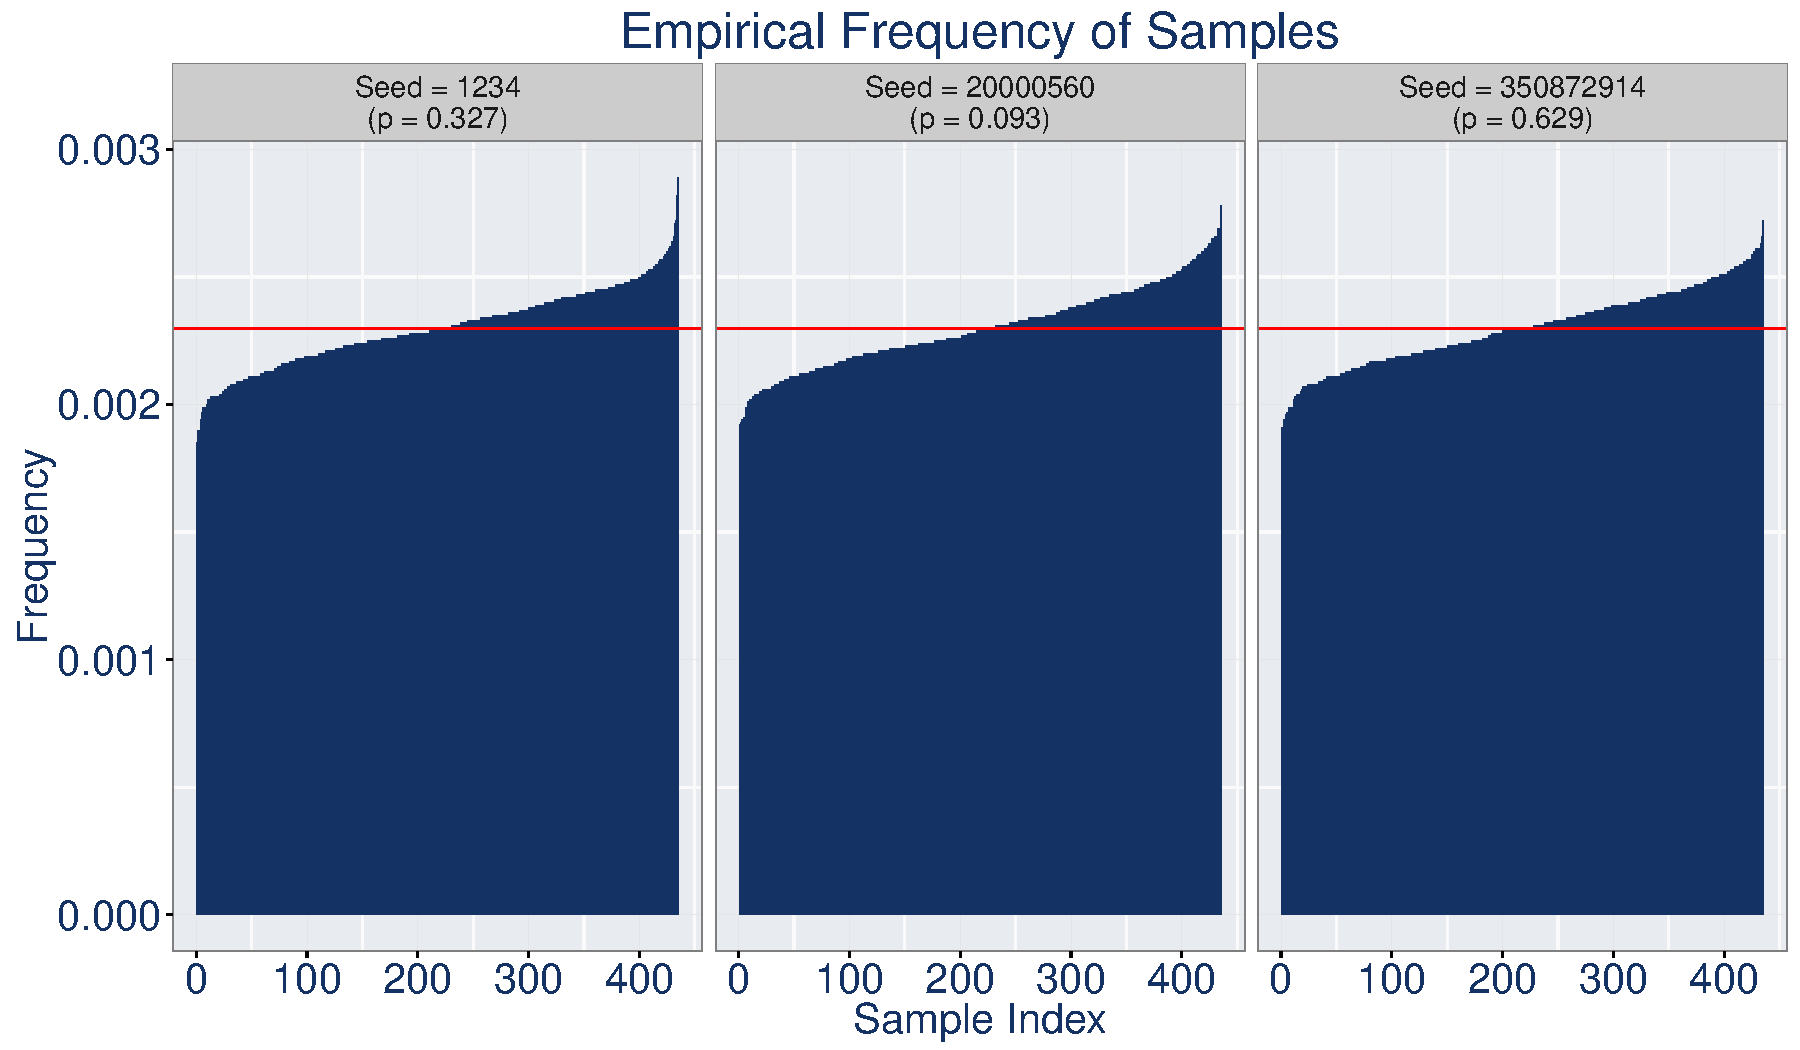
\includegraphics[width = 0.8\textwidth]{fig/bad-seeds.pdf}
%\end{center}
%\footnotesize{$10^5$ samples of size $2$ from a population of $30$ (Mersenne Twister in R)}
%\end{figure}
%}





\section[Common PRNGs]{Common PRNGs}

\frame{
\frametitle{Linear Congruential Generators}
LCGs have the form
$$ X_{n+1} = (a X_n + c) \mod m$$

Smart choices of $a$,$c$, and $m$ can make the LCG fast to compute and more or less random

\begin{theorem}[Hull-Dobell Full Period Theorem]
\label{thm:hull_dobell_period}
The period of an LCG is $m$ for all seeds $X_0$ if and only if
\begin{itemize}
\item $m$ and $c$ are relatively prime,
\item $a-1$ is divisible by all prime factors of $m$, and
\item $a-1$ is divisible by 4 if $m$ is divisible by 4.
\end{itemize}
\end{theorem}

}

\frame{
\frametitle{The good, the bad, and the ugly}
\begin{block}{(Knuth, 1997)}
``Random numbers should not be generated with a method chosen at random.''
\end{block}
\pause
\citet{marsaglia_random_1968} proved that $n$-tuples of numbers generated by any LCG will lie on parallel hyperplanes, making them especially non-random.


\begin{figure}[htbp]
\begin{center}
\includegraphics[width = 0.4\textwidth]{fig/randu.png}
\end{center}
     Triples of RANDU lie on 15 planes in 3D space \\ 
     $x_{n+1} = (65539 x_{n}) \mod 2^{31}$ \\
\footnotesize{(Wikipedia)}
\end{figure}
}

\frame{
\frametitle{Better LCGs}
\bit
\item Super-Duper: $X_{n+1} = (69069X_{n} )\mod 2^{32}$
\bit
\item $69069 = 3 \times 7 \times 11 \times 13 \times 23$
\item Considered a good LCG, passes spectral tests in low dimensions
\eit
\item MINSTD: $X_{n+1} = (16807 X_{n} )\mod (2^{31}-1)$
\bit
\item $16807 = 7^5$
\item The ``minimum standard'' against which other PRNGs should be judged (\cite{park_random_1988})
\eit
\item KISS: combines Super-Duper with two other PRNGs
\bit
\item Was previously the only PRNG in Stata
\item Period length over $2^{210}$
\eit
\item Wichman-Hill PRNG: a sum of 3 LCGs
\bit
\item Was previously the only PRNG in Excel
\item Faulty implementation didn't allow seeding and sometimes produced negative values (\cite{mccullough_microsoft_2008})
\eit
\eit

}


\frame{
\frametitle{Linear Congruential Generators}
\bit
\item Fast to compute and requires little memory
\item Some LCGs are more random than others -- depends on choosing good constants
\item Not unpredictable. We only need 2 values to determine the constants.
\item Possible to do jump ahead using mathematical formulas.
\eit
}



\frame{
\frametitle{Mersenne Twister (\cite{matsumoto_mersenne_1998})}



\begin{center}
\resizebox{10cm}{!}{    
\begin{tikzpicture}[node distance = 2cm, auto, scale = 0.25]
    % Place nodes
    \node [message] (m3) {$x_2$};
    \node [message, left of=m3] (m2) {$x_1$};
    \node [message, left of=m2] (m1) {$x_0$};
    \node [message, right of=m3, node distance=3cm] (mn1) {$x_{622}$};
    \node [message, right of=mn1] (mend) {$x_{623}$};
    \node [f, below of=m3, node distance = 1cm, minimum width = 5cm] (f) {Tempering};
    \node [io, below of = f, node distance = 1.5cm](output){Output};
    % Draw box around GLFSR
    \draw ($(m1.north west)+(-3,3)$)  rectangle ($(mend.south east)+(3,-0.5)$);
    % Draw edges
    \path [line] (m1) -- (m2);
    \path [line] (m2) -- (m3);
%    \path [line] (m1) -- (f);
%    \path [line] (m2) -- (f);
%    \path [line] (m3) -- (f);
%     \path [line] (mn1) -- (f);
%    \path [line] (mend) -- (f);
    \path [line,dashed] (m3) -- (mn1);
    \path [line] (mn1) -- (mend);
    \path [line] (f) -- (output);
    \draw[->, every node/.style={font=\sffamily\small}] (mend.north) -- ($(mend)+(0,2)$) -- ($(m1)+(0,2)$) node[above, pos=0.8] {GLFSR} -- (m1.north) ;
    \draw[->, every node/.style={font=\sffamily\small}] ($(mend.east)+(3,1)$) -- ($(mend.east)+(4,1)$) -- ($(mend.east)+(4,-4)$) -- (f.east) ;

\end{tikzpicture}
}
\end{center}

\bit
\item A ``twisted'' generalized linear feedback shift register: a complicated sequence of bitwise and linear operations
\item Enormous period of $2^{19937} - 1$, a Mersenne prime
\item $k$-distributed to 32-bit accuracy for $1 \leq k \leq 623$, i.e. tuples of up to length $623$ occur with equal frequency over the entire period
\item Integer seed is used to set the state, a $624 \times 32$ binary matrix
\eit 
}

\frame{
\frametitle{Mersenne Twister}
\bit
\item Fast to compute but has a large state space, not the most memory efficient
\item Fails some TestU01 tests but has been generally considered ``random'' enough for Statistics... (but stay tuned)
\item Completely predictable after we've seen 624 values
\item No good jump ahead feature
\eit
}



\frame{
\frametitle{A better alternative}

\textbf{One solution:} Find a class of PRNGs with infinite state space
}

\frame{
\frametitle{Hash function PRNGs}
\textbf{Hash functions} take in a message $x$ of arbitrary length and return a value $h(x)$ of fixed size (e.g. 256 bits)


\begin{center}
\resizebox{10cm}{!}{    
\begin{tikzpicture}[node distance = 1cm, auto, scale = 0.5]
    % Place nodes
    \node[io] (IV) {IV};
    \node [f, right of=IV] (f1) {f};
    \node [f, right of=f1] (f2) {f};
    \node [f, right of=f2, node distance=3cm] (fn1) {f};
    \node [f, right of=fn1] (fend) {f};
    \node [f, right of=fend] (g) {g};
    \node [io, right of=g] (hx) {$h(x)$};
    \node [message, above of=f1] (m1) {$x_1$};
    \node [message, above of=f2] (m2) {$x_2$};
    \node [message, above of=fn1] (mn1) {$x_{n-1}$};
    \node [message, above of=fend] (mend) {$x_n$};
    \node [message, above right = of m1, above left = of mend, minimum width = 5cm] (message) {$x$};
    % Draw edges
    \path [line] (IV) -- (f1);
    \path [line] (f1) -- (f2);
    \path [line] (message) -- (m1);
    \path [line] (message) -- (m2);
    \path [line] (message) -- (mn1);
    \path [line] (message) -- (mend);
    \draw [-,dotted] (m2) -- (mn1);
    \path [line] (m1) -- (f1);
    \path [line] (m2) -- (f2);
     \path [line] (mn1) -- (fn1);
    \path [line] (mend) -- (fend);
    \path [line] (fend) -- (g);
    \path [line,dashed] (f2) -- (fn1);
    \path [line] (fn1) -- (fend);
    \path [line] (g) -- (hx);
\end{tikzpicture}
}
\end{center}
Cryptographic hash functions:
\begin{itemize}
\item computationally infeasible to invert
\item difficult to find two inputs that map to the same output
\item small input changes produce large, unpredictable changes to output
\item resulting bits are uniformly distributed
\end{itemize}

}


\begin{frame}\label{sha256_procedure}
\frametitle{Hash function PRNGs}
Procedure for using a cryptographic hash function as PRNG:
\begin{enumerate}
\item Set a seed, a large random integer
\item Set the counter to $0$
\item Set the state to be ``seed,counter''
\item Hash the state value. This is your random number (expressed in hexadecimal).
\item Increment the counter
\item Repeat Steps 2-5 as many times as needed
\end{enumerate}

\vspace{15pt}
This PRNG passes the tests described. \hyperlink{sha256_tests}{\beamerbutton{see appendix}}
\end{frame}

\frame{
\frametitle{Hash function PRNGs}
\bit
\item Efficient: based on fast, pre-existing hash function code. Some cryptographic hash functions are even built into hardware (e.g. AES and Intel)
\item Memory efficient: only need to store the seed and counter
\item Unpredictable: small changes to input produce large unpredictable changes to output. The only way to figure out the sequence is to know the seed.
\item Jump ahead: add the desired number of steps to the counter
\eit
}

%  
%\frame{
%\frametitle{Simulations}
%\begin{figure}[htbp]
%\begin{center}
%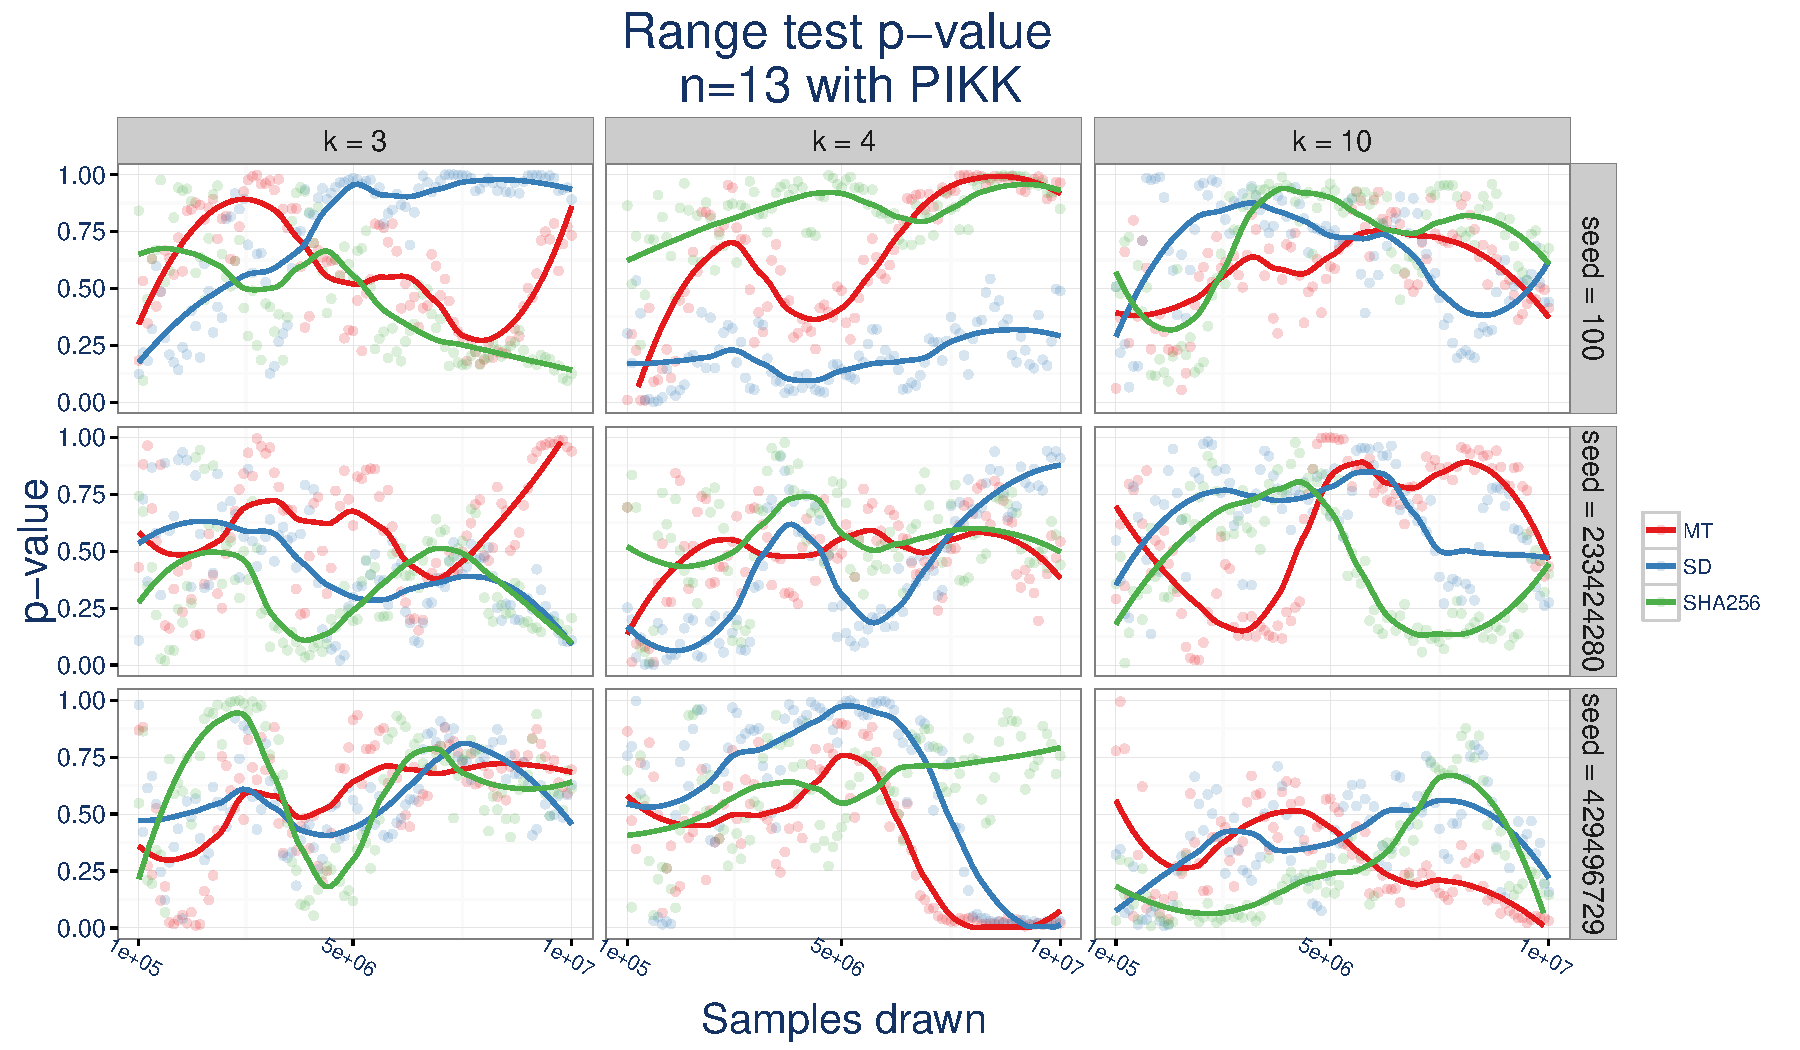
\includegraphics[width = \textwidth]{fig/prng-comparison-range-n13-pikk}
%\end{center}
%\end{figure}
%}
% 
%\frame{
%\frametitle{Simulations}
%\begin{figure}[htbp]
%\begin{center}
%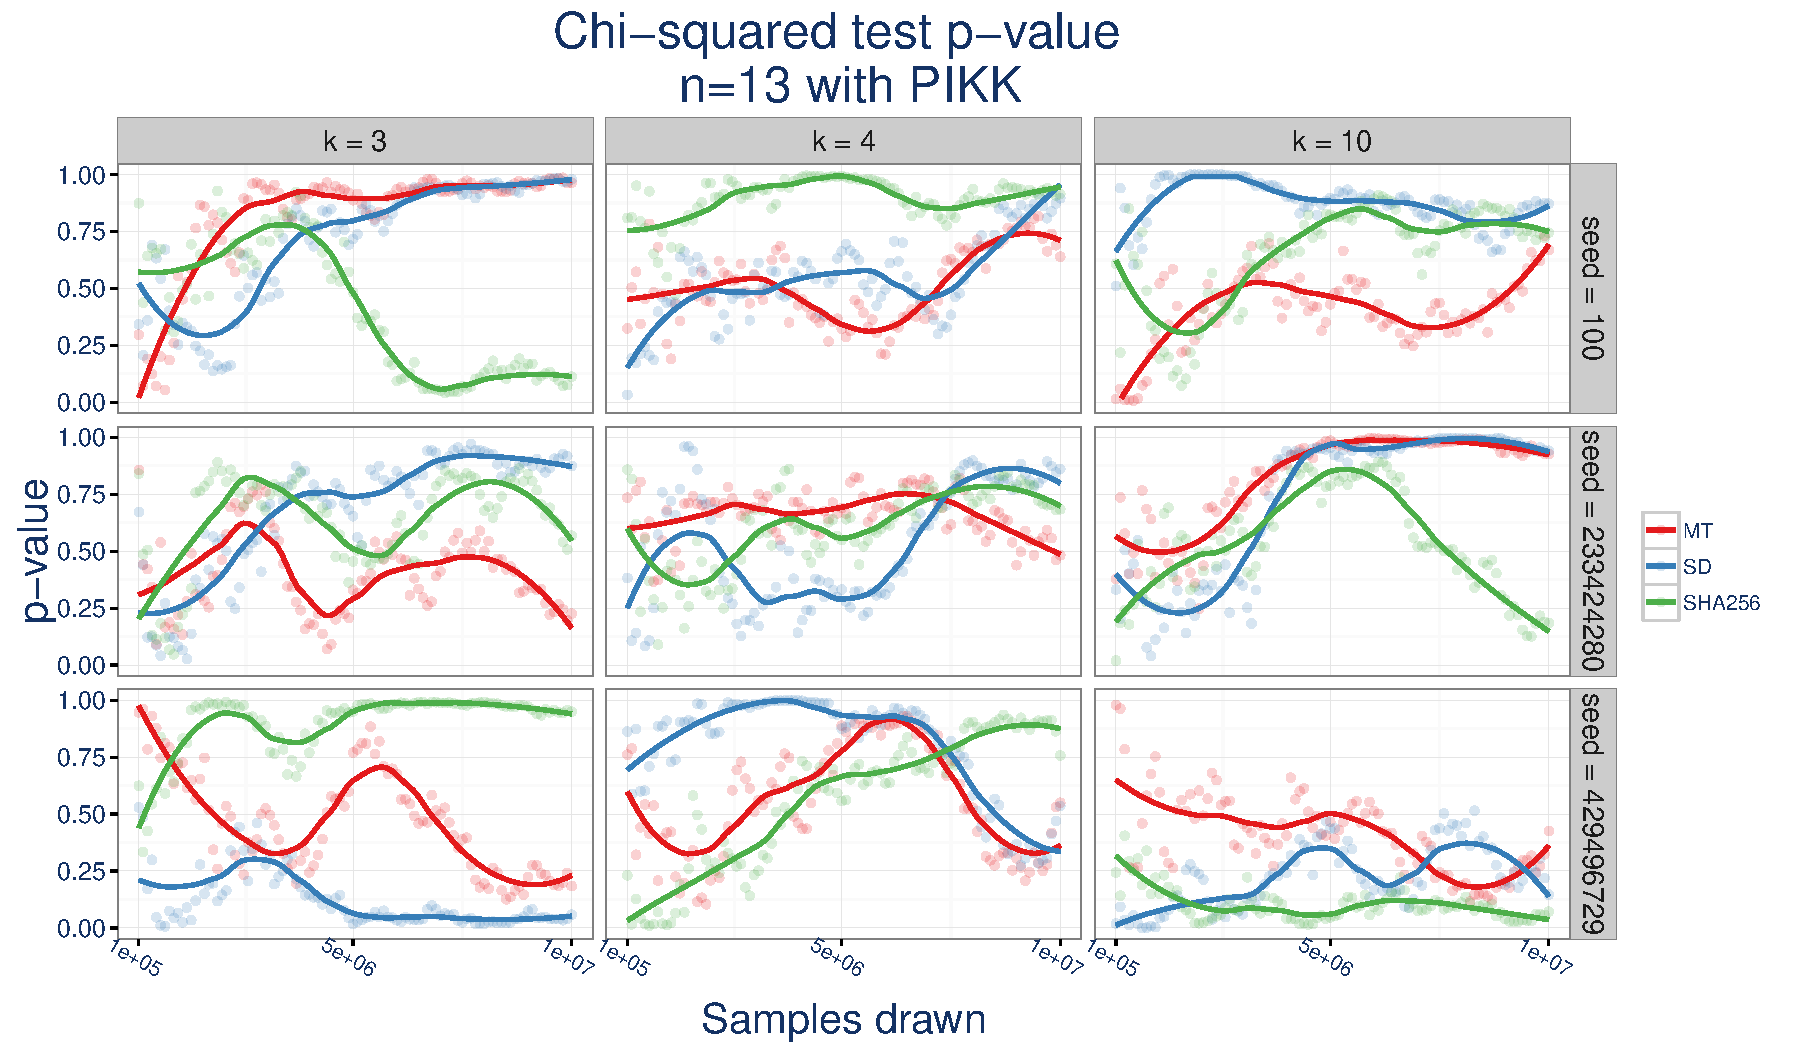
\includegraphics[width = \textwidth]{fig/prng-comparison-chisq-n13-pikk}
%\end{center}
%\end{figure}
%}

\frame{
\frametitle{Simulations}
\begin{figure}[htbp]
\begin{center}
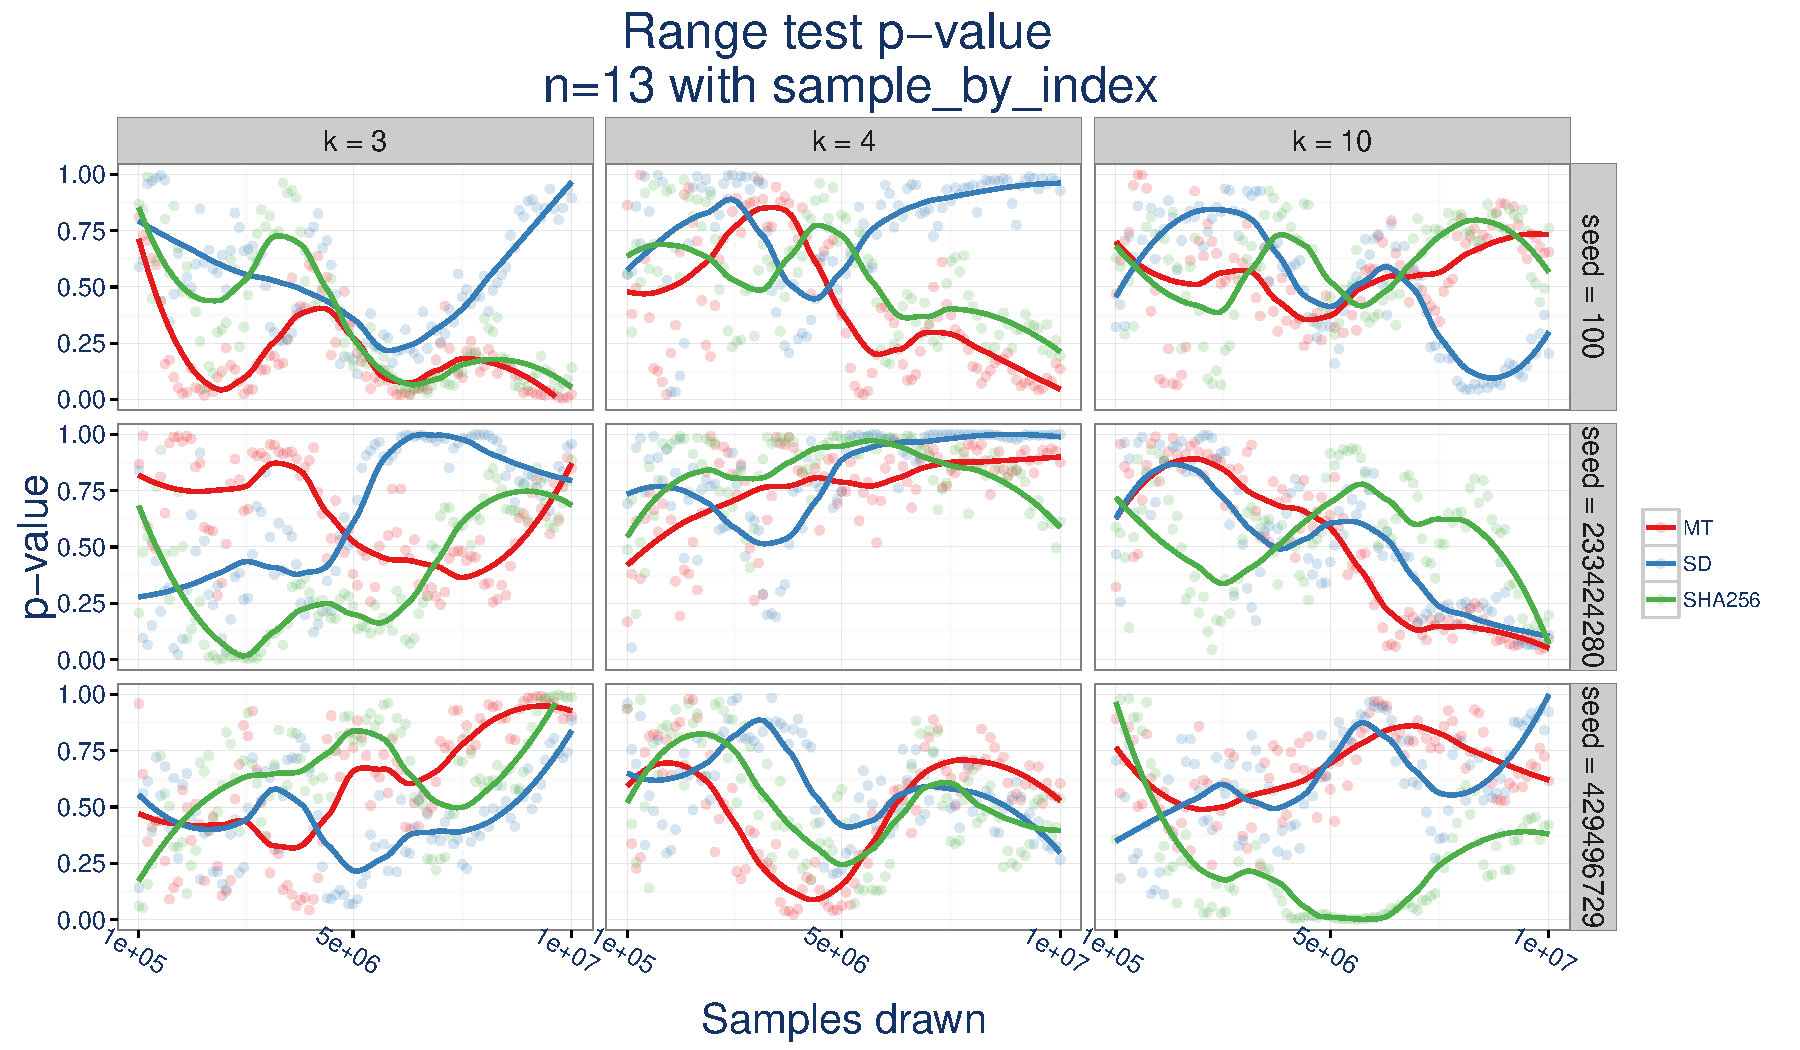
\includegraphics[width = \textwidth]{fig/prng-comparison-range-n13-sbi}
\end{center}
\end{figure}
}
 
\frame{
\frametitle{Simulations}
\begin{figure}[htbp]
\begin{center}
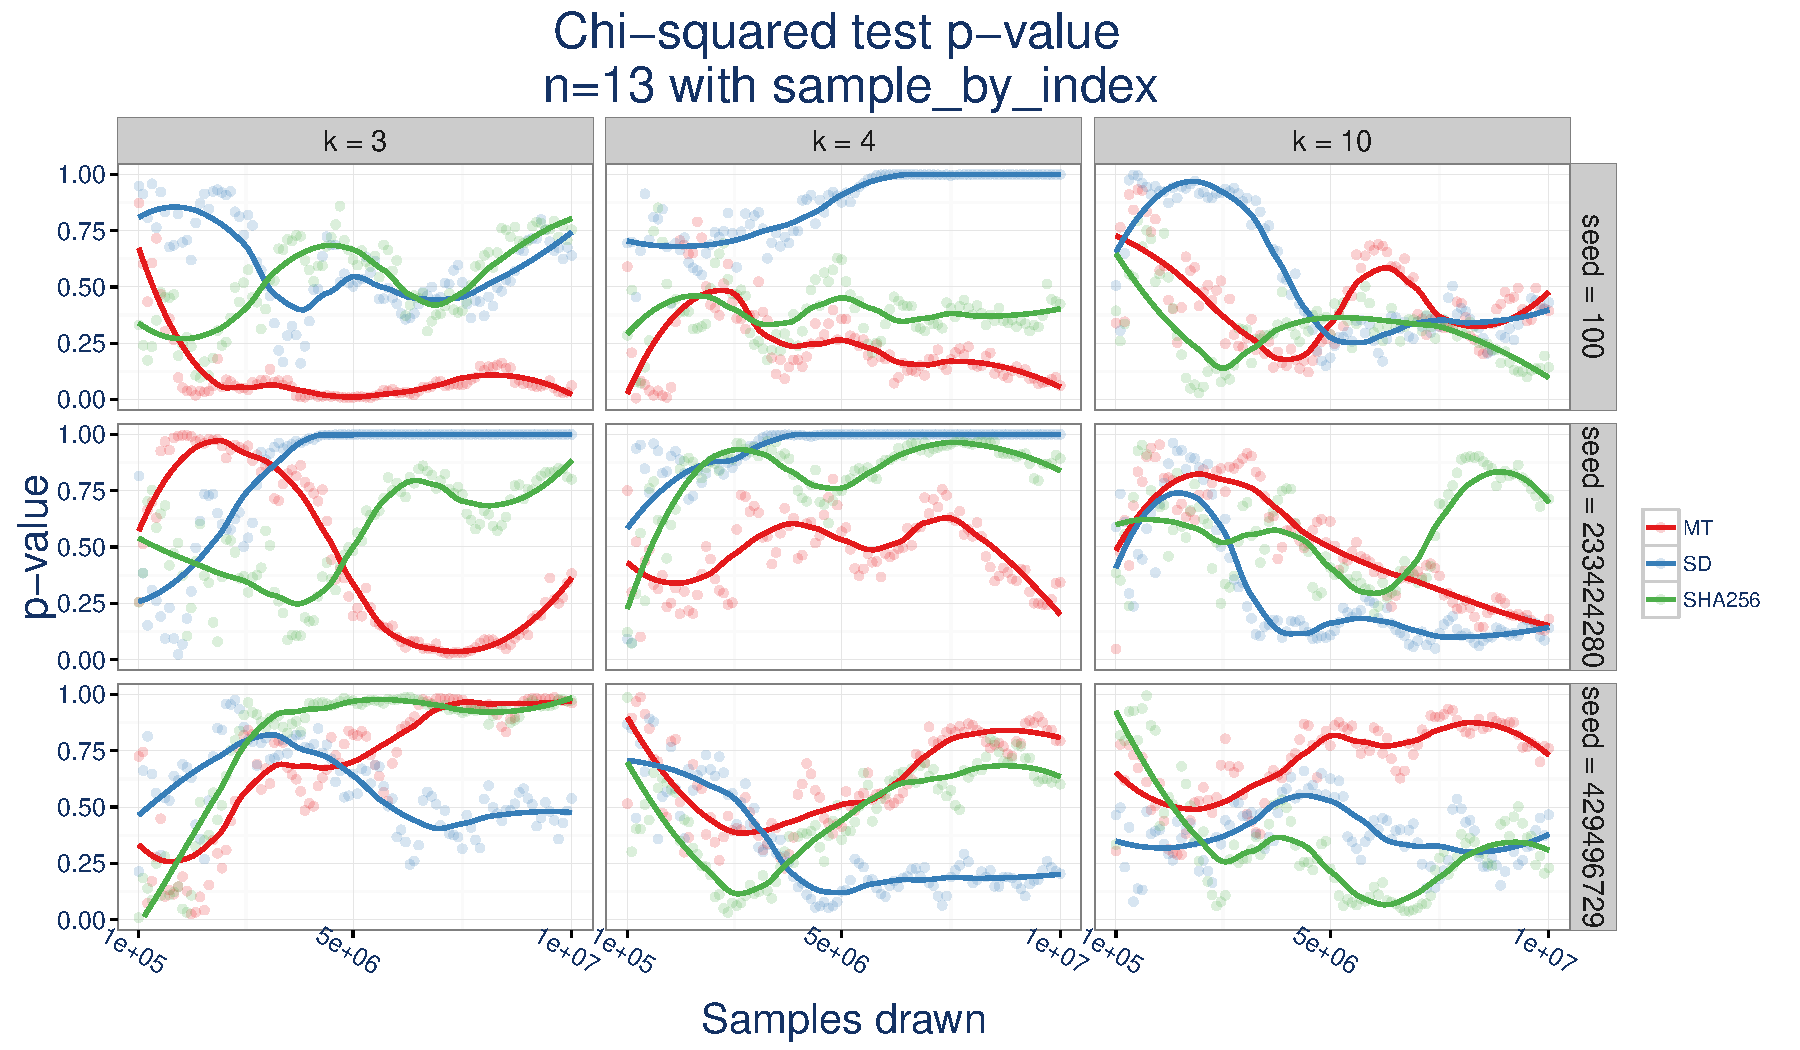
\includegraphics[width = \textwidth]{fig/prng-comparison-chisq-n13-sbi}
\end{center}
\end{figure}
}

\frame{
\frametitle{Simulations}
\todo{summarize sim results}
\bit
\item Even though sampling $k$ from $n$ is complementary to sampling $n-k$ from $n$, the resulting samples are not equally uniform
\item None of the 3 PRNGs is best overall -- results vary by seed value
\item $p$-value curves tend to dip around $5\times 10^6$ samples -- trade-off between statistical power and equidistribution of PRNG?
\eit
}

\frame{
\frametitle{Next steps}
%\todo{

Theoretical:
\bit
\item Study the properties of hash function PRNGs
\item Understand how the equidistribution of a PRNG relates to how uniformity of sampling frequencies over different segments of the period
\item Implement a sequential hypothesis test for uniformity of samples
\eit
Practical:
\bit
\item Find examples where results of a study would change from using a better SA/PRNG
\item Add these statistical tests to a more thorough test battery for PRNGs for Statistics
\item Create plug-in hash function PRNGs for R and Python
\eit
%}
}


\section[Appendix]{Appendix}


\begin{frame}[label = impossibility_bounds]
\frametitle{Impossibility bounds}
Let $F$ be the uniform distribution on all samples of size $k$ from a population of $n$.
For some subset of samples $S$,
define $\mathcal{G} = \{ G: G(S) = 0, S \in \mathcal{S}\}$ and $\nu = \lvert S \rvert$.


\begin{lemma}
For any $G \in \mathcal{G}$, $ \lVert F - G \rVert_1 \geq \frac{2\nu}{{n \choose k}}$
\end{lemma}


For any bounded function $\psi: \Omega \to \reals$ and for any $G \in \mathcal{G}$,

$$\left\lvert \int \psi dG - \int \psi dF \right\rvert \leq \lVert F - G \rVert_1 \lVert \psi \rVert_\infty$$


\begin{corollary}
There exists a statistic $\psi$ such that

$$\left\lvert  \ex_F(\psi) - \ex_G(\psi) \right\rvert \geq  \frac{2\nu \lVert \psi \rVert_\infty}{{n \choose k}}$$
\end{corollary}

\hyperlink{pigeonhole}{\beamerbutton{back}}

\end{frame}


\frame{
\tiny
\begin{proof}[Proof of Lemma]
Fix $S$ and choose $G \in \mathcal{G}$ such that $G(S) = 0, G(\omega) > 0$ for $\omega \in S^c$.
\begin{align*}
\lVert F - G \rVert_1 &= \sum_{\omega \in \Omega} \lvert F(\omega) - G(\omega) \rvert \\
&= \sum_{\omega \in S} \lvert F(\omega) - G(\omega) \rvert + \sum_{\omega \in S^c} \lvert F(\omega) - G(\omega) \rvert\\
&= \sum_{\omega \in S} \lvert F(\omega) \rvert + \sum_{\omega \in S^c} \lvert F(\omega) - G(\omega) \rvert\\
&= \frac{ \lvert S \rvert}{{n \choose k}}+ \sum_{\omega \in S^c} \lvert F(\omega) - (F(\omega) + \eps_\omega) \rvert\\
\end{align*}
\noindent where $\eps_\omega \in [ - {n \choose k}^{-1}, 1 - {n\choose k}^{-1}]$ and $\sum_{\omega \in S^c} \eps_\omega = \sum_{\omega \in S} F(\omega) =  \frac{ \lvert S \rvert}{{n \choose k}}$.
NB this must be the case to ensure that $\sum_{\omega} G(\omega) = 1$, since
$$\sum_{\omega} G(\omega) =\sum_{\omega\in S^c} G(\omega) = \sum_{\omega\in S^c} F(\omega) + \eps_\omega = \sum_{\omega\in S^c} F(\omega) + \sum_{\omega\in S} F(\omega) = 1.$$

Therefore,
\begin{align*}
\lVert F - G \rVert_1 &= \frac{ \lvert S \rvert}{{n \choose k}}+ \sum_{\omega \in S^c} \lvert \eps_\omega \rvert\\
&=  \frac{ \lvert S \rvert}{{n \choose k}}+ \sum_{\omega \in S} \lvert F(\omega) \\
&= \frac{2 \lvert S \rvert}{{n \choose k}}
\end{align*}
\end{proof}
\hyperlink{pigeonhole}{\beamerbutton{back}}
}

\begin{frame}[label = nonuniform-proof]
\tiny
\begin{proof}
Define $Y = \lfloor mX \rfloor + 1$ and $\tilde{X}$ to be a uniform random integer on $\{0, 1, \dots, 2^w - 1\}$ (while $X$ has the same distribution scaled by $2^{-w}$).
The selection probability for a particular integer value is 
\begin{align*}
\pr\left(Y = y\right) &= \pr\left(1 + \lfloor mX \rfloor = y\right) \\
&= \pr\left(y-1 \leq mX < y\right) \\
&= \pr\left(\tilde{X} < \frac{y2^w}{m}\right) - \pr\left(\tilde{X} < \frac{(y-1)2^w}{m}\right)\\
&= \pr\left(\tilde{X} < \left\lceil\frac{y2^w}{m}\right\rceil\right) - \pr\left(\tilde{X} \leq \left\lceil\frac{(y-1)2^w}{m}\right\rceil\right)\\
&= 2^{-w}\left(k^-(y)- k^-(y-1) + 1\right) = 2^{-w}\left(k^+(y-1)- k^-(y-1) \right)
\end{align*}

\noindent where, for fixed $m$, we define $k^-(i) \equiv \min \{k: k2^{-w} \geq i/m\}$ for all $i$,
$k^+(i) \equiv \max \{k : k2^{-w} < i/m \} = k^-(i+1)-1$ for $i = 0, \dots, m-1$
and $k^+(m) \equiv 2^w$.
The maximum ratio of selection probabilities is 

\begin{align*}
\max_{i, j \in \{0, \ldots, m-1\}} \frac{k^+(i) - k^-(i)}{k^+(j) - k^-(j)}
&= \frac{ \max_{i=0}^{m-1} (k^+(i) - k^-(i))}{\min_{i=0}^{m-1} (k^+(i) - k^-(i))} \\
&= \frac{ \max_{i=0}^{m-1} (k^+(i) - k^+(i+1) + 1)}{\min_{i=0}^{m-1} (k^-(i+1) - k^-(i) -1)} \\
&= \frac{\lceil 2^w/m \rceil + 1}{\lfloor 2^w/m \rfloor - 1} \\
&= 1 + 2^{-w}m + ...
\end{align*}

\end{proof}
\hyperlink{nonuniform-lemma}{\beamerbutton{back}}

\end{frame}


\begin{frame}\label{sha256_tests}

\todo{Insert table of p-values for several tests + several seeds}
\hyperlink{sha256_procedure}{\beamerbutton{back}}

\end{frame}



\begin{frame}
\frametitle{References}
\tiny
\bibliographystyle{plainnat}
\bibliography{refs}
\itemize
\end{frame}


\end{document}
